
\documentclass[addpoints]{exam}
% Used to insert images
\usepackage{graphicx}
\usepackage{color}

\printanswers

\newcommand{\event}{Dynamics}
\def\type{0}

\setlength\fillinlinelength{\textwidth}
\CorrectChoiceEmphasis{\color{red}\bfseries}
\SolutionEmphasis{\color{red}\bfseries}

\setlength\answerclearance{2pt}
\pagestyle{headandfoot}
% Adds a line to the top of the page
\runningheadrule
% The three braces correspond to the different parts of the header: the left is the top left text, middle is top middle, and right is top right.
\runningheader{\event}{\tournament}{\ifnum\type=1 Class Set Test \else Full Name:\hspace{1cm} \fi }
% Adds a line to the bottom of the page
\runningfootrule
% The three braces correspond to the different parts of the footer: the left is the bottom left text, middle is bottom middle, and right is bottom right.
% Doesn't include the title page in the page count 
% \runningfooter{}{Page \the\numexpr\thepage-1\   of \the\numexpr\numpages-1}{}
% Uncomment the line below if you want to include the title page in the page count 
\runningfooter{}{Page \thepage\   of \numpages}{}

\begin{document}
\begin{center}
    {\huge Grade 12 Physics \\ \event
    % Writes key if the answers are shown, otherwise writes test
    \ifprintanswers 
     \space Key
    \else 
     \space \ifnum\type<2 Test \fi \ifnum\type=1 \textbf{(CLASS SET)} \fi \ifnum\type=2 Answer Sheet \fi
    \fi \\ \vspace{3mm}\tournament\vspace{1mm}}
\end{center}
% Change to any picture or just some \vspace{.3\textheight} to leave it blank. [h] ensures that the image is placed in the same place in the document as in the code
\begin{figure}[h]
    \centering
    \includegraphics[height=.3\textheight, width=.6\textwidth, keepaspectratio]{}
\begin{figure}
    \centering
    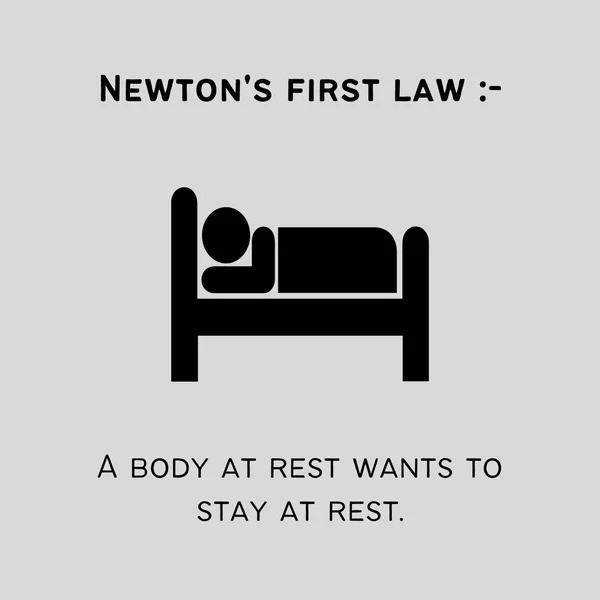
\includegraphics[width=0.5\linewidth]{kinematics-sleep.jpg}
    \label{fig:enter-label}
\end{figure}
\end{figure}


\begin{center}
    First Name: \ifprintanswers
    \underline{\hspace{3.5cm}}\textbf{KEY}\underline{\hspace{5.5cm}}\\\vspace{5mm}
    \else
        \underline{\hspace{10cm}}\\ \vspace{5mm}
    \fi
    Last Name: \underline{\hspace{10cm}}\\ \vspace{5mm}

\end{center}

% Change the list below to reflect the instructions for your test
\noindent\textbf{\underline{Directions:}}
\begin{itemize}
    % If the test is a class set, an instruction will appear to not write on the test paper.
    \ifnum\type=1 \item \textbf{This test is a class set.} Please do not write any answers on this paper. \fi
    % Adds an instruction 
    \item Please answer to 2 decimal points
    \item The test is designed to be completed in 75 minutes
\end{itemize}
\begin{center}
\textit{For grading use only}\\

\multirowgradetable{1}[pages]   
\end{center}

\newpage
\begin{questions}

\section*{Questions}

\question[1] A car accelerates uniformly from rest to a speed of 25 m/s in 10 seconds. What is the car's acceleration?
\begin{choices}
    \choice 1.5 m/s$^2$
    \correctchoice 2.5 m/s$^2$
    \choice 3.5 m/s$^2$
    \choice 4.5 m/s$^2$
\end{choices}

\question[1] A projectile is launched with an initial velocity of 20 m/s at an angle of 30$^\circ$ above the horizontal. What is the maximum height it reaches?
\begin{choices}
    \choice 10 m
    \choice 15 m
    \correctchoice 20 m
    \choice 25 m
\end{choices}

\question[1] What is the force required to accelerate a 5 kg object at 3 m/s$^2$?
\begin{choices}
    \correctchoice 15 N
    \choice 10 N
    \choice 20 N
    \choice 25 N
\end{choices}

\question[1] An object moves in a circular path with a radius of 4 m at a constant speed of 8 m/s. What is the centripetal acceleration?
\begin{choices}
    \choice 8 m/s$^2$
    \choice 16 m/s$^2$
    \correctchoice 16 m/s$^2$
    \choice 32 m/s$^2$
\end{choices}

\question[1] A spring with a spring constant of 200 N/m is compressed by 0.1 m. What is the potential energy stored in the spring?
\begin{choices}
    \choice 1 J
    \choice 2 J
    \correctchoice 1 J
    \choice 4 J
\end{choices}

\question[1] A 10 kg object is dropped from a height of 20 m. What is its speed just before it hits the ground? (Assume no air resistance)
\begin{choices}
    \choice 10 m/s
    \choice 14 m/s
    \correctchoice 20 m/s
    \choice 25 m/s
\end{choices}

\question[1] A 3-ohm resistor is connected to a 12 V battery. What is the current flowing through the resistor?
\begin{choices}
    \choice 2 A
    \correctchoice 4 A
    \choice 6 A
    \choice 8 A
\end{choices}

\question[1] A 2 kg object is moving with a velocity of 5 m/s. What is its kinetic energy?
\begin{choices}
    \choice 25 J
    \choice 15 J
    \correctchoice 25 J
    \choice 50 J
\end{choices}

\question[1] A 50 N force is applied to a 10 kg object, causing it to accelerate. What is the object's acceleration?
\begin{choices}
    \choice 2 m/s$^2$
    \choice 5 m/s$^2$
    \correctchoice 5 m/s$^2$
    \choice 10 m/s$^2$
\end{choices}

\question[1] A block slides down a frictionless incline of 30$^\circ$. What is the acceleration of the block along the incline?
\begin{choices}
    \choice 3.3 m/s$^2$
    \correctchoice 5.0 m/s$^2$
    \choice 7.5 m/s$^2$
    \choice 9.8 m/s$^2$
\end{choices}




\section*{Short Answer}

\question A football with a mass of 0.4 kg is thrown with an initial velocity of 20 m/s at an angle of 30° above the horizontal.
\begin{parts}
    \part[5] Calculate the time it will take for the football to reach its maximum height.
    \part[5] Find the maximum height of the football.
    \part[5] Determine the total time the football will be in the air before landing.
    \part[5] Calculate the horizontal distance it will cover before landing.
\end{parts}
\begin{solution}[5cm]
\textbf{(a) The time it will take for the football to reach its maximum height:}

The vertical component of the initial velocity is given by:
\[
v_{y0} = v_0 \sin \theta = 20 \sin 30^\circ = 10 \, \text{m/s}
\]
The time to reach the maximum height is calculated using:
\[
t_{\text{max height}} = \frac{v_{y0}}{g} = \frac{10}{9.8} \approx 1.02 \, \text{seconds}
\]

\textbf{(b) The maximum height of the football:}

The maximum height is given by the equation:
\[
h_{\text{max}} = \frac{v_{y0}^2}{2g} = \frac{10^2}{2 \times 9.8} = \frac{100}{19.6} \approx 5.10 \, \text{meters}
\]

\textbf{(c) The total time the football will be in the air before landing:}

The total time in the air is twice the time to reach the maximum height:
\[
t_{\text{total}} = 2 \times t_{\text{max height}} = 2 \times 1.02 \approx 2.04 \, \text{seconds}
\]

\textbf{(d) The horizontal distance the football will cover before landing:}

The horizontal velocity is given by:
\[
v_{x} = v_0 \cos \theta = 20 \cos 30^\circ \approx 17.32 \, \text{m/s}
\]
The horizontal distance is:
\[
d = v_{x} \times t_{\text{total}} = 17.32 \times 2.04 \approx 35.3 \, \text{meters}
\]
\end{solution}



\question A block of mass 4 kg rests on an inclined plane with an angle of 20° to the horizontal. The block is connected by a rope to a hanging block of mass 2 kg. The coefficient of friction between the block on the incline and the surface is 0.11.
\begin{parts}
    \part[5] Calculate the normal force acting on the block on the incline.
    \part[5] Find the frictional force acting on the block on the incline.
    \part[5] Calculate the tension in the rope.
    \part[5] Determine the acceleration of the system.
\end{parts}
\begin{solution}[5cm]
\textbf{(a) The normal force acting on the block on the incline:}

The normal force is calculated as:
\[
F_{\text{N}} = m_1 g \cos \theta = 4 \times 9.8 \times \cos 20^\circ \approx 36.8 \, \text{N}
\]

\textbf{(b) The frictional force acting on the block on the incline:}

The frictional force is given by:
\[
F_{\text{friction}} = \mu F_{\text{N}} = 0.11 \times 36.8 \approx 4.05 \, \text{N}
\]

\textbf{(c) The tension in the rope:}

First, calculate the force due to gravity acting on the hanging block:
\[
F_{\text{gravity}} = m_2 g = 2 \times 9.8 = 19.6 \, \text{N}
\]
The net force on the system is:
\[
F_{\text{net}} = F_{\text{gravity}} - F_{\text{friction}} - m_1 g \sin \theta = 19.6 - 4.05 - 4 \times 9.8 \times \sin 20^\circ
\]
\[
F_{\text{net}} \approx 19.6 - 4.05 - 13.4 = 2.15 \, \text{N}
\]
The tension in the rope is:
\[
T = F_{\text{net}} = 2.15 \, \text{N}
\]

\textbf{(d) The acceleration of the system:}

The total mass of the system is:
\[
m_{\text{total}} = m_1 + m_2 = 4 + 2 = 6 \, \text{kg}
\]
Using Newton's second law:
\[
a = \frac{F_{\text{net}}}{m_{\text{total}}} = \frac{2.15}{6} \approx 0.36 \, \text{m/s}^2
\]
\end{solution}



\question A canoe is traveling at a velocity of 60.0 km/h due south with respect to the water. Due to a current, the canoe ends up traveling at 30.0 km/h at an angle of 45° south of west with respect to the shore.
\begin{parts}
    \part[5] Using vector components, calculate the velocity of the current.
    \part[5] Find the direction of the current with respect to the southward direction.
\end{parts}
\begin{solution}[5cm]
\textbf{(a) The velocity of the current:}

We know the velocity of the canoe with respect to the shore is \( \vec{v}_{\text{canoe/shore}} = 30.0 \, \text{km/h} \, [S 45^\circ W] \), and the velocity of the canoe with respect to the water is \( \vec{v}_{\text{canoe/water}} = 60.0 \, \text{km/h} \, [S] \).

First, decompose both velocities into their vector components:

\[
\vec{v}_{\text{canoe/shore}, x} = 30.0 \, \text{km/h} \cdot \sin(45^\circ) \approx 21.2 \, \text{km/h},
\]
\[
\vec{v}_{\text{canoe/shore}, y} = -30.0 \, \text{km/h} \cdot \cos(45^\circ) \approx -21.2 \, \text{km/h}.
\]

For the canoe with respect to the water, the components are:

\[
\vec{v}_{\text{canoe/water}, x} = 0 \, \text{km/h},
\]
\[
\vec{v}_{\text{canoe/water}, y} = -60.0 \, \text{km/h}.
\]

Now calculate the velocity of the current using the equation:

\[
\vec{v}_{\text{current}} = \vec{v}_{\text{canoe/shore}} - \vec{v}_{\text{canoe/water}}.
\]

Substitute the components:

\[
\vec{v}_{\text{current}, x} = 21.2 - 0 = 21.2 \, \text{km/h},
\]
\[
\vec{v}_{\text{current}, y} = -21.2 - (-60.0) = 38.8 \, \text{km/h}.
\]

Thus, the velocity of the current is:

\[
\vec{v}_{\text{current}} = \langle 21.2, 38.8 \rangle \, \text{km/h}.
\]

\textbf{(b) The direction of the current with respect to the southward direction:}

The direction of the current is given by:

\[
\theta = \tan^{-1}\left(\frac{v_{\text{current}, x}}{v_{\text{current}, y}}\right) = \tan^{-1}\left(\frac{21.2}{38.8}\right) \approx 29.7^\circ.
\]

Thus, the current is directed \( 29.7^\circ \) east of south.

\textbf{Final answers:}
\begin{itemize}
    \item (a) The velocity of the current is \( \vec{v}_{\text{current}} = \langle 21.2, 38.8 \rangle \, \text{km/h} \).
    \item (b) The direction of the current is \( 29.7^\circ \) east of south.
\end{itemize}

\end{solution}



\question A 0.050 kg yo-yo is swung in a vertical circle on the end of its 0.30 m long string. The yo-yo is at its slowest speed, just enough to complete the vertical circle.
\begin{parts}
    \part[5] Calculate the minimum speed of the yo-yo required to complete the circle.
    \part[5] Draw a labelled free-body diagram at the highest point of the vertical circle.
    \part[5] What will the maximum tension in the string be when the yo-yo is swung at the minimum speed?
    \part[5] Where will the maximum tension occur in the vertical circle? Draw a labelled free-body diagram showing the forces acting on the yo-yo at this point.
\end{parts}
\begin{solution}[5cm]
\textbf{(a) The minimum speed required to complete the circle:}

At the highest point of the vertical circle, the tension in the string is zero. The centripetal force is provided by the gravitational force:

\[
F_{\text{centripetal}} = \frac{m v_{\text{min}}^2}{r}.
\]

At the highest point, the gravitational force is equal to the centripetal force:

\[
m g = \frac{m v_{\text{min}}^2}{r}.
\]

Canceling out the mass \( m \) from both sides:

\[
g = \frac{v_{\text{min}}^2}{r}.
\]

Solving for \( v_{\text{min}} \):

\[
v_{\text{min}} = \sqrt{g r} = \sqrt{9.8 \times 0.30} = \sqrt{2.94} \approx 1.71 \, \text{m/s}.
\]

\textbf{(b) Free-body diagram at the highest point:}

At the highest point, the forces acting on the yo-yo are:
\begin{itemize}
    \item The tension \( T \) in the string acting upward.
    \item The gravitational force \( mg \) acting downward.
\end{itemize}
The free-body diagram would show these forces.

\textbf{(c) The maximum tension in the string:}

The maximum tension occurs at the lowest point of the vertical circle. The tension must balance the gravitational force and provide the centripetal force. The total tension is:

\[
T_{\text{max}} = \frac{m v_{\text{min}}^2}{r} + m g.
\]

Substitute the known values:

\[
T_{\text{max}} = \frac{0.050 \times (1.71)^2}{0.30} + 0.050 \times 9.8.
\]

\[
T_{\text{max}} = \frac{0.050 \times 2.9241}{0.30} + 0.490 = 0.487 + 0.490 = 0.977 \, \text{N}.
\]

\textbf{(d) The maximum tension occurs at the lowest point:}

The maximum tension occurs at the lowest point of the vertical circle, where the forces acting on the yo-yo are:
\begin{itemize}
    \item The tension \( T \) acting upward.
    \item The gravitational force \( mg \) acting downward.
\end{itemize}
The free-body diagram at this point would show the tension vector pointing upward and the gravitational force vector pointing downward.

\textbf{Final answers:}
\begin{itemize}
    \item (a) The minimum speed required to complete the circle is \( v_{\text{min}} = 1.71 \, \text{m/s} \).
    \item (b) The free-body diagram at the highest point shows tension upward and gravity downward.
    \item (c) The maximum tension in the string is \( T_{\text{max}} = 0.977 \, \text{N} \).
    \item (d) The maximum tension occurs at the lowest point, where the forces are tension upward and gravity downward.
\end{itemize}
\end{solution}



\question A 5 kg block rests on an inclined plane with a 30° angle. The block is connected by a rope to a 3 kg hanging block. The coefficient of friction between the 5 kg block and the plane is 0.15.
\begin{parts}
    \part[5] Determine the gravitational force acting on the 5 kg block.
    \part[5] Calculate the frictional force acting on the 5 kg block.
    \part[5] Find the tension in the rope connecting the blocks.
    \part[5] Calculate the acceleration of the system.
\end{parts}
\begin{solution}[5cm]
\textbf{(a) The gravitational force acting on the 5 kg block:}

The gravitational force acting on the block is given by:

\[
F_{\text{gravity}} = m g = 5 \times 9.8 = 49 \, \text{N}.
\]

Thus, the gravitational force acting on the 5 kg block is \( 49 \, \text{N} \).

\textbf{(b) The frictional force acting on the 5 kg block:}

The frictional force is calculated using the formula:

\[
F_{\text{friction}} = \mu F_{\text{N}},
\]
where \( \mu = 0.15 \) is the coefficient of friction and \( F_{\text{N}} \) is the normal force.

The normal force can be found by:

\[
F_{\text{N}} = m g \cos \theta = 5 \times 9.8 \times \cos 30^\circ \approx 5 \times 9.8 \times 0.866 = 42.5 \, \text{N}.
\]

Now calculate the frictional force:

\[
F_{\text{friction}} = 0.15 \times 42.5 \approx 6.375 \, \text{N}.
\]

Thus, the frictional force acting on the 5 kg block is \( 6.375 \, \text{N} \).

\textbf{Final answers:}
\begin{itemize}
    \item (a) The gravitational force acting on the 5 kg block is \( 49 \, \text{N} \).
    \item (b) The frictional force acting on the 5 kg block is \( 6.375 \, \text{N} \).
\end{itemize}
\end{solution}



\question A boat is crossing a river that is 200 m wide. The boat has a velocity of 8 m/s relative to the water, and the current in the river flows at a velocity of 3 m/s.
\begin{parts}
    \part[5] Calculate the time it takes for the boat to cross the river.
    \part[5] Determine the distance the boat will be displaced downstream while crossing.
    \part[5] Calculate the angle at which the boat must head to travel directly across the river (i.e., without drifting downstream).
\end{parts}
\begin{solution}[5cm]
\textbf{(a) The time it takes for the boat to cross the river:}

To calculate the time it takes for the boat to cross the river, we use the formula:

\[
\text{Time} = \frac{\text{Width of the river}}{\text{Velocity of the boat relative to the water}}.
\]

Given that the width of the river is 200 m and the velocity of the boat relative to the water is 8 m/s:

\[
\text{Time} = \frac{200}{8} = 25 \, \text{seconds}.
\]

Thus, the time it takes for the boat to cross the river is \( 25 \, \text{seconds} \).

\textbf{(b) The distance the boat will be displaced downstream:}

The downstream displacement is calculated using the velocity of the current and the time it takes the boat to cross the river:

\[
\text{Displacement} = \text{Velocity of current} \times \text{Time}.
\]

Given that the velocity of the current is 3 m/s and the time taken to cross is 25 seconds:

\[
\text{Displacement} = 3 \times 25 = 75 \, \text{m}.
\]

Thus, the boat will be displaced 75 m downstream while crossing the river.

\textbf{(c) The angle at which the boat must head to travel directly across the river:}

To travel directly across the river, the boat must head at an angle that compensates for the current. The angle \( \theta \) is found using:

\[
\tan \theta = \frac{\text{Velocity of current}}{\text{Velocity of boat relative to the water}}.
\]

Substitute the given values:

\[
\tan \theta = \frac{3}{8} \approx 0.375.
\]

Solving for \( \theta \):

\[
\theta = \tan^{-1}(0.375) \approx 20.56^\circ.
\]

Thus, the boat must head at an angle of approximately \( 20.56^\circ \) upstream to travel directly across the river.

\textbf{Final answers:}
\begin{itemize}
    \item (a) The time it takes for the boat to cross the river is \( 25 \, \text{seconds} \).
    \item (b) The distance the boat will be displaced downstream is \( 75 \, \text{m} \).
    \item (c) The angle at which the boat must head to travel directly across the river is \( 20.56^\circ \) upstream.
\end{itemize}
\end{solution}

\end{questions}

\end{document}
